\documentclass[11pt]{article}

\newcommand{\titrechapitre}{Variables aléatoires -- Exercices}
\newcommand{\titreclasse}{Lycée Jean-Baptiste \textsc{Corot}}
\newcommand{\pagination}{\thepage}%{\thepage/\pageref{LastPage}}
\newcommand{\topbotmargins}{2cm}
\newcommand{\spacebelowexo}{3mm}
%%%%%%%%%%%%%%%%%%%%%%%%%%%%%%%%%%%%%%%%%%%%%%%%%%%%%%%%%%%%%%%%%%%%%%%%%%%%%%%%
%
% PACKAGES
% ========
%
%%%%%%%%%%%%%%%%%%%%%%%%%%%%%%%%%%%%%%%%%%%%%%%%%%%%%%%%%%%%%%%%%%%%%%%%%%%%%%%%

\usepackage[english, french]{babel}
\usepackage[utf8]{inputenc}
\usepackage[T1]{fontenc}
\usepackage{graphicx}
\usepackage{amsmath,amssymb,amsthm,amsopn}
\usepackage{hyperref}

% Pour avoir l'écriture \mathscr (math script)
% ============================================

\usepackage{mathrsfs}

% Deal with coma as a decimal separator
% =====================================

\usepackage{icomma}

% Package Geometry
% ================

\usepackage[a4paper, lmargin=2cm, rmargin=2cm, top=\topbotmargins, bottom=\topbotmargins]{geometry}

% Package multicol
% ================

\usepackage{multicol}

% Redefine abstract
% =================

% Note
% ====
%
% Le reste a été commenté pour ne pas charger trop de choses au démarrage. On
% verra si on en a besoin plus tard.
%
% --------
%
%\usepackage{mathrsfs}
%\usepackage{multirow}
%\usepackage{bm}
%\hypersetup{
%    colorlinks=true,
%    linkcolor=blue,
%    citecolor=red,
%}
%\usepackage{diagbox}
%
%\usepackage{algorithm}
%\usepackage{algpseudocode}
%
%\renewcommand{\algorithmicrequire}{\textbf{Input:}}
%\renewcommand{\algorithmicensure}{\textbf{Output:}}


%%%%%%%%%%%%%%%%%%%%%%%%%%%%%%%%%%%%%%%%%%%%%%%%%%%%%%%%%%%%%%%%%%%%%%%%%%%%%%%%
%
% TIKZ
% ====
%
%%%%%%%%%%%%%%%%%%%%%%%%%%%%%%%%%%%%%%%%%%%%%%%%%%%%%%%%%%%%%%%%%%%%%%%%%%%%%%%%

\usepackage{tikz}
\usetikzlibrary{arrows}

\usepackage{tkz-tab} % Variation tables

\usepackage{pgfplots}
%\usepackage{pgf-pie} % Pie charts

\pgfplotsset{
%\newcommand{\settingsgraph}{
x=.5cm,y=.5cm,
xticklabel style = {font=\scriptsize, yshift=.1cm},
yticklabel style = {font=\scriptsize, xshift=.1cm},
axis lines=middle,
ymajorgrids=true,
xmajorgrids=true,
major grid style = {color=white!80!blue},
xmin=-5.5,
xmax=5.5,
ymin=-5.5,
ymax=5.5,
xtick={-5.0,-4.0,...,5.0},
ytick={-5.0,-4.0,...,5.0},
}

% Tikz style

\tikzset{round/.style={circle, draw=black, very thick, scale = 0.7}}
\tikzset{arrow/.style={->, >=latex}}
\tikzset{dashed-arrow/.style={->, >=latex, dashed}}

\newcommand{\point}[3]{\draw[very thick, #3] (#1-.1, #2)--(#1+.1, #2)
(#1, #2-.1)--(#1, #2+.1)}

%%%%%%%%%%%%%%%%%%%%%%%%%%%%%%%%%%%%%%%%%%%%%%%%%%%%%%%%%%%%%%%%%%%%%%%%%%%%%%%%
%
% FANCY HEADER
% ============
%
%%%%%%%%%%%%%%%%%%%%%%%%%%%%%%%%%%%%%%%%%%%%%%%%%%%%%%%%%%%%%%%%%%%%%%%%%%%%%%%%


\usepackage{fancyhdr}
\usepackage{lastpage}

\pagestyle{fancy}
\newcommand{\changefont}{\fontsize{9}{9}\selectfont}
\renewcommand{\headrulewidth}{0mm}
\renewcommand{\footrulewidth}{0mm}

\fancyhead[C]{}
\fancyhead[L]{\titreclasse}
\fancyhead[R]{\titrechapitre}
\fancyfoot[C]{}
\fancyfoot[L]{}
\fancyfoot[R]{\pagination}
\addtolength{\skip\footins}{20pt} % distance between text and footnotes

%%%%%%%%%%%%%%%%%%%%%%%%%%%%%%%%%%%%%%%%%%%%%%%%%%%%%%%%%%%%%%%%%%%%%%%%%%%%%%%%
%
% THEOREM STYLE
% =============
%
%%%%%%%%%%%%%%%%%%%%%%%%%%%%%%%%%%%%%%%%%%%%%%%%%%%%%%%%%%%%%%%%%%%%%%%%%%%%%%%%

\usepackage[tikz]{bclogo}
\usepackage{mdframed}

\usepackage{tcolorbox}
\tcbuselibrary{listings, breakable, theorems, skins}

%\newtheoremstyle{break}%
%{}{}%
%{\itshape}{}%
%{\bfseries}{}%  % Note that final punctuation is omitted.
%{\newline}{}

\newtheoremstyle{scbf}%
{}{}%
{}{}%
%{\scshape}{}%  % Note that final punctuation is omitted.
{\bfseries\scshape}{}%  % Note that final punctuation is omitted.
{\newline}{}

%\theoremstyle{break}
%\theoremstyle{plain}
%\newtheorem{thm}{Theorem}[section]
%\newtheorem{lm}[thm]{Lemma}
%\newtheorem{prop}[thm]{Proposition}
%\newtheorem{cor}[thm]{Corollary}

%\theoremstyle{scbf}
%\newtheorem{exo}{$\star$ Exercice}

%\theoremstyle{definition}
%\newtheorem{defi}[thm]{Definition}
%\newtheorem{ex}[thm]{Example}

%\theoremstyle{remark}
%\newtheorem{rem}[thm]{Remark}

% Defining the Remark environment
% ===============================

\newenvironment{rmq}
  {
    \begin{bclogo}[logo=\bcinfo, noborder=true]{Remarque}
  }
  {
    \end{bclogo}
  }

% Defining the exercise environment
% =================================

\newcounter{exos}
\setcounter{exos}{1}

\newenvironment{exo}
  {
    \begin{bclogo}[logo=\bccrayon, noborder=true]{Exercice \theexos}
  }
  {
    \end{bclogo}
    \addtocounter{exos}{1}
  }


% Redefining the proof environment from amsthm
% ============================================

\tcolorboxenvironment{proof}{
  blanker, breakable, before skip=10pt,after skip=10pt,
  borderline west={1mm}{0pt}{red},
  left=5mm,
}

% Defining the definition environment
% ===================================

\colorlet{coldef}{black!50!green}

\newcounter{defis}
\setcounter{defis}{1}

\newenvironment{defi}[1]
  {
    \begin{defihid}{{#1}}{\thedefis}
  }
  {
    \end{defihid}
    \addtocounter{defis}{1}
  }

\newtcolorbox{defihid}[2]{%
  empty,title={ {\bfseries Définition {#2}} ({#1})},attach boxed title to top left,
boxed title style={empty,size=minimal,toprule=2pt,top=4pt,
overlay={\draw[coldef,line width=2pt]
([yshift=-1pt]frame.north west)--([yshift=-1pt]frame.north east);}},
coltitle=coldef,
before=\par\medskip\noindent,parbox=false,boxsep=0pt,left=0pt,right=3mm,top=4pt,
breakable,pad at break*=0mm,vfill before first,
overlay unbroken={\draw[coldef,line width=1pt]
([yshift=-1pt]title.north east)--([xshift=-0.5pt,yshift=-1pt]title.north-|frame.east)
--([xshift=-0.5pt]frame.south east)--(frame.south west); },
overlay first={\draw[coldef,line width=1pt]
([yshift=-1pt]title.north east)--([xshift=-0.5pt,yshift=-1pt]title.north-|frame.east)
--([xshift=-0.5pt]frame.south east); },
overlay middle={\draw[coldef,line width=1pt] ([xshift=-0.5pt]frame.north east)
--([xshift=-0.5pt]frame.south east); },
overlay last={\draw[coldef,line width=1pt] ([xshift=-0.5pt]frame.north east)
--([xshift=-0.5pt]frame.south east)--(frame.south west);},%
}

\newenvironment{notation}
  {
    \begin{notationhid}{\thedefis}
  }
  {
    \end{notationhid}
    \addtocounter{defis}{1}
  }

\newtcolorbox{notationhid}[1]{%
  empty,title={Notation {#1}},attach boxed title to top left,
boxed title style={empty,size=minimal,toprule=2pt,top=4pt,
overlay={\draw[coldef,line width=2pt]
([yshift=-1pt]frame.north west)--([yshift=-1pt]frame.north east);}},
coltitle=coldef,fonttitle=\bfseries,
before=\par\medskip\noindent,parbox=false,boxsep=0pt,left=0pt,right=3mm,top=4pt,
breakable,pad at break*=0mm,vfill before first,
overlay unbroken={\draw[coldef,line width=1pt]
([yshift=-1pt]title.north east)--([xshift=-0.5pt,yshift=-1pt]title.north-|frame.east)
--([xshift=-0.5pt]frame.south east)--(frame.south west); },
overlay first={\draw[coldef,line width=1pt]
([yshift=-1pt]title.north east)--([xshift=-0.5pt,yshift=-1pt]title.north-|frame.east)
--([xshift=-0.5pt]frame.south east); },
overlay middle={\draw[coldef,line width=1pt] ([xshift=-0.5pt]frame.north east)
--([xshift=-0.5pt]frame.south east); },
overlay last={\draw[coldef,line width=1pt] ([xshift=-0.5pt]frame.north east)
--([xshift=-0.5pt]frame.south east)--(frame.south west);},%
}


% Defining the proposition, theorem, etc. environment
% ===================================================

\colorlet{colprop}{red!75!black}

\newcounter{props}
\setcounter{props}{1}

\newenvironment{prop}
  {
    \begin{prophid}{\theprops}
  }
  {
    \end{prophid}
    \refstepcounter{props}
  }

\newtcolorbox{prophid}[1]{%
empty,title={Propriété {#1}},attach boxed title to top left,
boxed title style={empty,size=minimal,toprule=2pt,top=4pt,
overlay={\draw[colprop,line width=2pt]
([yshift=-1pt]frame.north west)--([yshift=-1pt]frame.north east);}},
coltitle=colprop,fonttitle=\bfseries,
before=\par\medskip\noindent,parbox=false,boxsep=0pt,left=0pt,right=3mm,top=4pt,
breakable,pad at break*=0mm,vfill before first,
overlay unbroken={\draw[colprop,line width=1pt]
([yshift=-1pt]title.north east)--([xshift=-0.5pt,yshift=-1pt]title.north-|frame.east)
--([xshift=-0.5pt]frame.south east)--(frame.south west); },
overlay first={\draw[colprop,line width=1pt]
([yshift=-1pt]title.north east)--([xshift=-0.5pt,yshift=-1pt]title.north-|frame.east)
--([xshift=-0.5pt]frame.south east); },
overlay middle={\draw[colprop,line width=1pt] ([xshift=-0.5pt]frame.north east)
--([xshift=-0.5pt]frame.south east); },
overlay last={\draw[colprop,line width=1pt] ([xshift=-0.5pt]frame.north east)
--([xshift=-0.5pt]frame.south east)--(frame.south west);},%
}

\newenvironment{propadm}
  {
    \begin{propadmhid}{\theprops}
  }
  {
    \end{propadmhid}
    \refstepcounter{props}
  }

  \newtcolorbox{propadmhid}[1]{%
    empty,title={{\bfseries Propriété {#1}} (admise)},attach boxed title to top left,
boxed title style={empty,size=minimal,toprule=2pt,top=4pt,
overlay={\draw[colprop,line width=2pt]
([yshift=-1pt]frame.north west)--([yshift=-1pt]frame.north east);}},
coltitle=colprop,%fonttitle=\bfseries,
before=\par\medskip\noindent,parbox=false,boxsep=0pt,left=0pt,right=3mm,top=4pt,
breakable,pad at break*=0mm,vfill before first,
overlay unbroken={\draw[colprop,line width=1pt]
([yshift=-1pt]title.north east)--([xshift=-0.5pt,yshift=-1pt]title.north-|frame.east)
--([xshift=-0.5pt]frame.south east)--(frame.south west); },
overlay first={\draw[colprop,line width=1pt]
([yshift=-1pt]title.north east)--([xshift=-0.5pt,yshift=-1pt]title.north-|frame.east)
--([xshift=-0.5pt]frame.south east); },
overlay middle={\draw[colprop,line width=1pt] ([xshift=-0.5pt]frame.north east)
--([xshift=-0.5pt]frame.south east); },
overlay last={\draw[colprop,line width=1pt] ([xshift=-0.5pt]frame.north east)
--([xshift=-0.5pt]frame.south east)--(frame.south west);},%
}

\newenvironment{propnom}[1]
  {
    \begin{propnomhid}{#1}{\theprops}
  }
  {
    \end{propnomhid}
    \refstepcounter{props}
  }

\newtcolorbox{propnomhid}[2]{%
empty,title={{\bfseries Propriété {#2}} ({#1})},attach boxed title to top left,
boxed title style={empty,size=minimal,toprule=2pt,top=4pt,
overlay={\draw[colprop,line width=2pt]
([yshift=-1pt]frame.north west)--([yshift=-1pt]frame.north east);}},
coltitle=colprop,
before=\par\medskip\noindent,parbox=false,boxsep=0pt,left=0pt,right=3mm,top=4pt,
breakable,pad at break*=0mm,vfill before first,
overlay unbroken={\draw[colprop,line width=1pt]
([yshift=-1pt]title.north east)--([xshift=-0.5pt,yshift=-1pt]title.north-|frame.east)
--([xshift=-0.5pt]frame.south east)--(frame.south west); },
overlay first={\draw[colprop,line width=1pt]
([yshift=-1pt]title.north east)--([xshift=-0.5pt,yshift=-1pt]title.north-|frame.east)
--([xshift=-0.5pt]frame.south east); },
overlay middle={\draw[colprop,line width=1pt] ([xshift=-0.5pt]frame.north east)
--([xshift=-0.5pt]frame.south east); },
overlay last={\draw[colprop,line width=1pt] ([xshift=-0.5pt]frame.north east)
--([xshift=-0.5pt]frame.south east)--(frame.south west);},%
}




\newenvironment{thm}
  {
    \begin{thmhid}{\theprops}
  }
  {
    \end{thmhid}
    \refstepcounter{props}
  }

\newtcolorbox{thmhid}[1]{%
empty,title={Théorème {#1}},attach boxed title to top left,
boxed title style={empty,size=minimal,toprule=2pt,top=4pt,
overlay={\draw[colprop,line width=2pt]
([yshift=-1pt]frame.north west)--([yshift=-1pt]frame.north east);}},
coltitle=colprop,fonttitle=\bfseries,
before=\par\medskip\noindent,parbox=false,boxsep=0pt,left=0pt,right=3mm,top=4pt,
breakable,pad at break*=0mm,vfill before first,
overlay unbroken={\draw[colprop,line width=1pt]
([yshift=-1pt]title.north east)--([xshift=-0.5pt,yshift=-1pt]title.north-|frame.east)
--([xshift=-0.5pt]frame.south east)--(frame.south west); },
overlay first={\draw[colprop,line width=1pt]
([yshift=-1pt]title.north east)--([xshift=-0.5pt,yshift=-1pt]title.north-|frame.east)
--([xshift=-0.5pt]frame.south east); },
overlay middle={\draw[colprop,line width=1pt] ([xshift=-0.5pt]frame.north east)
--([xshift=-0.5pt]frame.south east); },
overlay last={\draw[colprop,line width=1pt] ([xshift=-0.5pt]frame.north east)
--([xshift=-0.5pt]frame.south east)--(frame.south west);},%
}

\newenvironment{thmadm}
  {
    \begin{thmadmhid}{\theprops}
  }
  {
    \end{thmadmhid}
    \refstepcounter{props}
  }

  \newtcolorbox{thmadmhid}[1]{%
    empty,title={{\bfseries Théorème {#1}} (admis)},attach boxed title to top left,
boxed title style={empty,size=minimal,toprule=2pt,top=4pt,
overlay={\draw[colprop,line width=2pt]
([yshift=-1pt]frame.north west)--([yshift=-1pt]frame.north east);}},
coltitle=colprop,%fonttitle=\bfseries,
before=\par\medskip\noindent,parbox=false,boxsep=0pt,left=0pt,right=3mm,top=4pt,
breakable,pad at break*=0mm,vfill before first,
overlay unbroken={\draw[colprop,line width=1pt]
([yshift=-1pt]title.north east)--([xshift=-0.5pt,yshift=-1pt]title.north-|frame.east)
--([xshift=-0.5pt]frame.south east)--(frame.south west); },
overlay first={\draw[colprop,line width=1pt]
([yshift=-1pt]title.north east)--([xshift=-0.5pt,yshift=-1pt]title.north-|frame.east)
--([xshift=-0.5pt]frame.south east); },
overlay middle={\draw[colprop,line width=1pt] ([xshift=-0.5pt]frame.north east)
--([xshift=-0.5pt]frame.south east); },
overlay last={\draw[colprop,line width=1pt] ([xshift=-0.5pt]frame.north east)
--([xshift=-0.5pt]frame.south east)--(frame.south west);},%
}

\newenvironment{thmnom}[1]
  {
    \begin{thmnomhid}{#1}{\theprops}
  }
  {
    \end{thmnomhid}
    \refstepcounter{props}
  }

\newtcolorbox{thmnomhid}[2]{%
empty,title={{\bfseries Théorème {#2}} ({#1})},attach boxed title to top left,
boxed title style={empty,size=minimal,toprule=2pt,top=4pt,
overlay={\draw[colprop,line width=2pt]
([yshift=-1pt]frame.north west)--([yshift=-1pt]frame.north east);}},
coltitle=colprop,
before=\par\medskip\noindent,parbox=false,boxsep=0pt,left=0pt,right=3mm,top=4pt,
breakable,pad at break*=0mm,vfill before first,
overlay unbroken={\draw[colprop,line width=1pt]
([yshift=-1pt]title.north east)--([xshift=-0.5pt,yshift=-1pt]title.north-|frame.east)
--([xshift=-0.5pt]frame.south east)--(frame.south west); },
overlay first={\draw[colprop,line width=1pt]
([yshift=-1pt]title.north east)--([xshift=-0.5pt,yshift=-1pt]title.north-|frame.east)
--([xshift=-0.5pt]frame.south east); },
overlay middle={\draw[colprop,line width=1pt] ([xshift=-0.5pt]frame.north east)
--([xshift=-0.5pt]frame.south east); },
overlay last={\draw[colprop,line width=1pt] ([xshift=-0.5pt]frame.north east)
--([xshift=-0.5pt]frame.south east)--(frame.south west);},%
}

\newenvironment{coro}
  {
    \begin{corohid}{\theprops}
  }
  {
    \end{corohid}
    \refstepcounter{props}
  }

  \newtcolorbox{corohid}[1]{%
  empty,title={Corollaire {#1}},attach boxed title to top left,
boxed title style={empty,size=minimal,toprule=2pt,top=4pt,
overlay={\draw[colprop,line width=2pt]
([yshift=-1pt]frame.north west)--([yshift=-1pt]frame.north east);}},
coltitle=colprop,fonttitle=\bfseries,
before=\par\medskip\noindent,parbox=false,boxsep=0pt,left=0pt,right=3mm,top=4pt,
breakable,pad at break*=0mm,vfill before first,
overlay unbroken={\draw[colprop,line width=1pt]
([yshift=-1pt]title.north east)--([xshift=-0.5pt,yshift=-1pt]title.north-|frame.east)
--([xshift=-0.5pt]frame.south east)--(frame.south west); },
overlay first={\draw[colprop,line width=1pt]
([yshift=-1pt]title.north east)--([xshift=-0.5pt,yshift=-1pt]title.north-|frame.east)
--([xshift=-0.5pt]frame.south east); },
overlay middle={\draw[colprop,line width=1pt] ([xshift=-0.5pt]frame.north east)
--([xshift=-0.5pt]frame.south east); },
overlay last={\draw[colprop,line width=1pt] ([xshift=-0.5pt]frame.north east)
--([xshift=-0.5pt]frame.south east)--(frame.south west);},%
}

\newenvironment{lemme}
  {
    \begin{lemmehid}{\theprops}
  }
  {
    \end{lemmehid}
    \refstepcounter{props}
  }

  \newtcolorbox{lemmehid}[1]{%
  empty,title={Lemme {#1}},attach boxed title to top left,
boxed title style={empty,size=minimal,toprule=2pt,top=4pt,
overlay={\draw[colprop,line width=2pt]
([yshift=-1pt]frame.north west)--([yshift=-1pt]frame.north east);}},
coltitle=colprop,fonttitle=\bfseries,
before=\par\medskip\noindent,parbox=false,boxsep=0pt,left=0pt,right=3mm,top=4pt,
breakable,pad at break*=0mm,vfill before first,
overlay unbroken={\draw[colprop,line width=1pt]
([yshift=-1pt]title.north east)--([xshift=-0.5pt,yshift=-1pt]title.north-|frame.east)
--([xshift=-0.5pt]frame.south east)--(frame.south west); },
overlay first={\draw[colprop,line width=1pt]
([yshift=-1pt]title.north east)--([xshift=-0.5pt,yshift=-1pt]title.north-|frame.east)
--([xshift=-0.5pt]frame.south east); },
overlay middle={\draw[colprop,line width=1pt] ([xshift=-0.5pt]frame.north east)
--([xshift=-0.5pt]frame.south east); },
overlay last={\draw[colprop,line width=1pt] ([xshift=-0.5pt]frame.north east)
--([xshift=-0.5pt]frame.south east)--(frame.south west);},%
}

\colorlet{colexemple}{blue!50!black}
%\newtcolorbox{exemple}{empty, title=Exemple, attach boxed title to top left,
%  boxed title style={empty, size=minimal, toprule=2pt, top=4pt,
%    overlay={\draw[colexemple,line width=2pt]
%([yshift=-1pt]frame.north west)--([yshift=-1pt]frame.north east);}},
%coltitle=colexemple,fonttitle=\bfseries,%\large\bfseries,
%before=\par\medskip\noindent,parbox=false,boxsep=0pt,left=0pt,right=3mm,top=4pt,
%overlay={\draw[colexemple,line width=1pt]
%([yshift=-1pt]title.north east)--([xshift=-0.5pt,yshift=-1pt]title.north-|frame.east)
%--([xshift=-0.5pt]frame.south east)--(frame.south west); },
%}

\newcounter{exemples}
\setcounter{exemples}{1}

\newenvironment{exemple}
  {
    \begin{exemplehid}{\theexemples}
  }
  {
    \end{exemplehid}
    \addtocounter{exemples}{1}
  }

\newtcolorbox{exemplehid}[1]{%
empty,title={Exemple {#1}},attach boxed title to top left,
boxed title style={empty,size=minimal,toprule=2pt,top=4pt,
overlay={\draw[colexemple,line width=2pt]
([yshift=-1pt]frame.north west)--([yshift=-1pt]frame.north east);}},
coltitle=colexemple,fonttitle=\bfseries,
before=\par\medskip\noindent,parbox=false,boxsep=0pt,left=0pt,right=3mm,top=4pt,
breakable,pad at break*=0mm,vfill before first,
overlay unbroken={\draw[colexemple,line width=1pt]
([yshift=-1pt]title.north east)--([xshift=-0.5pt,yshift=-1pt]title.north-|frame.east)
--([xshift=-0.5pt]frame.south east)--(frame.south west); },
overlay first={\draw[colexemple,line width=1pt]
([yshift=-1pt]title.north east)--([xshift=-0.5pt,yshift=-1pt]title.north-|frame.east)
--([xshift=-0.5pt]frame.south east); },
overlay middle={\draw[colexemple,line width=1pt] ([xshift=-0.5pt]frame.north east)
--([xshift=-0.5pt]frame.south east); },
overlay last={\draw[colexemple,line width=1pt] ([xshift=-0.5pt]frame.north east)
--([xshift=-0.5pt]frame.south east)--(frame.south west);},%
}

\newenvironment{contrex}
  {
    \begin{contrexhid}{\theexemples}
  }
  {
    \end{contrexhid}
    \addtocounter{exemples}{1}
  }

\newtcolorbox{contrexhid}[1]{%
empty,title={Contre-exemple {#1}},attach boxed title to top left,
boxed title style={empty,size=minimal,toprule=2pt,top=4pt,
overlay={\draw[colexemple,line width=2pt]
([yshift=-1pt]frame.north west)--([yshift=-1pt]frame.north east);}},
coltitle=colexemple,fonttitle=\bfseries,
before=\par\medskip\noindent,parbox=false,boxsep=0pt,left=0pt,right=3mm,top=4pt,
breakable,pad at break*=0mm,vfill before first,
overlay unbroken={\draw[colexemple,line width=1pt]
([yshift=-1pt]title.north east)--([xshift=-0.5pt,yshift=-1pt]title.north-|frame.east)
--([xshift=-0.5pt]frame.south east)--(frame.south west); },
overlay first={\draw[colexemple,line width=1pt]
([yshift=-1pt]title.north east)--([xshift=-0.5pt,yshift=-1pt]title.north-|frame.east)
--([xshift=-0.5pt]frame.south east); },
overlay middle={\draw[colexemple,line width=1pt] ([xshift=-0.5pt]frame.north east)
--([xshift=-0.5pt]frame.south east); },
overlay last={\draw[colexemple,line width=1pt] ([xshift=-0.5pt]frame.north east)
--([xshift=-0.5pt]frame.south east)--(frame.south west);},%
}

\newenvironment{app}
  {
    \begin{apphid}{\theexemples}
  }
  {
    \end{apphid}
    \addtocounter{exemples}{1}
  }

\newtcolorbox{apphid}[1]{%
empty,title={Application {#1}},attach boxed title to top left,
boxed title style={empty,size=minimal,toprule=2pt,top=4pt,
overlay={\draw[colexemple,line width=2pt]
([yshift=-1pt]frame.north west)--([yshift=-1pt]frame.north east);}},
coltitle=colexemple,fonttitle=\bfseries,
before=\par\medskip\noindent,parbox=false,boxsep=0pt,left=0pt,right=3mm,top=4pt,
breakable,pad at break*=0mm,vfill before first,
overlay unbroken={\draw[colexemple,line width=1pt]
([yshift=-1pt]title.north east)--([xshift=-0.5pt,yshift=-1pt]title.north-|frame.east)
--([xshift=-0.5pt]frame.south east)--(frame.south west); },
overlay first={\draw[colexemple,line width=1pt]
([yshift=-1pt]title.north east)--([xshift=-0.5pt,yshift=-1pt]title.north-|frame.east)
--([xshift=-0.5pt]frame.south east); },
overlay middle={\draw[colexemple,line width=1pt] ([xshift=-0.5pt]frame.north east)
--([xshift=-0.5pt]frame.south east); },
overlay last={\draw[colexemple,line width=1pt] ([xshift=-0.5pt]frame.north east)
--([xshift=-0.5pt]frame.south east)--(frame.south west);},%
}

%%%%%%%%%%%%%%%%%%%%%%%%%%%%%%%%%%%%%%%%%%%%%%%%%%%%%%%%%%%%%%%%%%%%%%%%%%%%%%%%
%
% ENUMERATE
% =========
%
%%%%%%%%%%%%%%%%%%%%%%%%%%%%%%%%%%%%%%%%%%%%%%%%%%%%%%%%%%%%%%%%%%%%%%%%%%%%%%%%

\usepackage{enumerate}
\usepackage{enumitem}

% To have special enumerate items like
%
% 1/
% 2/
% 3/

%%%%%%%%%%%%%%%%%%%%%%%%%%%%%%%%%%%%%%%%%%%%%%%%%%%%%%%%%%%%%%%%%%%%%%%%%%%%%%%%
%
% ARRAYS
% ======
%
%%%%%%%%%%%%%%%%%%%%%%%%%%%%%%%%%%%%%%%%%%%%%%%%%%%%%%%%%%%%%%%%%%%%%%%%%%%%%%%%


\usepackage{array}
\usepackage{makecell} % Used to break lines within arrays
\usepackage{multirow}
\usepackage{booktabs} % Used to have nice arrays with headrules

%%%%%%%%%%%%%%%%%%%%%%%%%%%%%%%%%%%%%%%%%%%%%%%%%%%%%%%%%%%%%%%%%%%%%%%%%%%%%%%%
%
% WRITE CODE
% ==========
%
%%%%%%%%%%%%%%%%%%%%%%%%%%%%%%%%%%%%%%%%%%%%%%%%%%%%%%%%%%%%%%%%%%%%%%%%%%%%%%%%

\usepackage{listings}
\usepackage{xcolor}

%New colors defined below
\definecolor{codegreen}{rgb}{0,0.6,0}
\definecolor{codegray}{rgb}{0.5,0.5,0.5}
\definecolor{codepurple}{rgb}{0.58,0,0.82}
\definecolor{backcolour}{rgb}{0.95,0.95,0.92}

%Code listing style named "mystyle"
\lstdefinestyle{python}{
  %backgroundcolor=\color{backcolour},
  commentstyle=\color{codegreen},
  keywordstyle=\color{magenta},
  numberstyle=\tiny\color{codegray},
  stringstyle=\color{codepurple},
  basicstyle=\ttfamily\footnotesize,
  breakatwhitespace=false,
  breaklines=true,
  captionpos=b,
  keepspaces=true,
  numbers=left,
  numbersep=5pt,
  showspaces=false,
  showstringspaces=false,
  showtabs=false,
  tabsize=2
}

\lstset{style=python}

%%%%%%%%%%%%%%%%%%%%%%%%%%%%%%%%%%%%%%%%%%%%%%%%%%%%%%%%%%%%%%%%%%%%%%%%%%%%%%%%
%
% Tabular 
% =======
%
%%%%%%%%%%%%%%%%%%%%%%%%%%%%%%%%%%%%%%%%%%%%%%%%%%%%%%%%%%%%%%%%%%%%%%%%%%%%%%%%

% In order to obtain a tabular with given width.

\usepackage{tabularx}
\newcolumntype{Y}{>{\centering\arraybackslash}X}
\newcolumntype{R}{>{\raggedright\arraybackslash}X}
\newcolumntype{L}{>{\raggedleft\arraybackslash}X}
% \usepackage{tabulary} % younger brother

%%%%%%%%%%%%%%%%%%%%%%%%%%%%%%%%%%%%%%%%%%%%%%%%%%%%%%%%%%%%%%%%%%%%%%%%%%%%%%%%
%
% MACROS
% ======
%
%%%%%%%%%%%%%%%%%%%%%%%%%%%%%%%%%%%%%%%%%%%%%%%%%%%%%%%%%%%%%%%%%%%%%%%%%%%%%%%%

% Math Operators

\DeclareMathOperator{\Card}{Card}
\DeclareMathOperator{\Gal}{Gal}
\DeclareMathOperator{\Id}{Id}
\DeclareMathOperator{\Img}{Im}
\DeclareMathOperator{\Ker}{Ker}
\DeclareMathOperator{\Minpoly}{Minpoly}
\DeclareMathOperator{\Mod}{mod}
\DeclareMathOperator{\Ord}{Ord}
\DeclareMathOperator{\ppcm}{ppcm}
\DeclareMathOperator{\pgcd}{pgcd}
\DeclareMathOperator{\tr}{Tr}
\DeclareMathOperator{\Vect}{Vect}
\DeclareMathOperator{\Span}{Span}
\DeclareMathOperator{\rank}{rank}
\DeclareMathOperator{\rg}{rg}
\DeclareMathOperator{\ev}{ev}
\DeclareMathOperator{\Var}{Var}

% Shortcuts

\newcommand{\eg}{\emph{e.g. }}
\newcommand{\ent}[2]{[\![#1,#2]\!]}
\newcommand{\ie}{\emph{i.e. }}
\newcommand{\ps}[2]{\left\langle#1,#2\right\rangle}
\newcommand{\eqdef}{\overset{\text{def}}{=}}
\newcommand{\E}{\mathcal{E}}
\newcommand{\M}{\mathcal{M}}
\newcommand{\A}{\mathcal{A}}
\newcommand{\B}{\mathcal{B}}
\newcommand{\R}{\mathcal{R}}
\newcommand{\D}{\mathcal{D}}
\newcommand{\Pcal}{\mathcal{P}}
\newcommand{\K}{\mathbf{k}}
\newcommand{\vect}[1]{\overrightarrow{#1}}



\begin{document}
%\maketitle\thispagestyle{fancy}

\begin{exo}
On lance un dé équilibré comportant $6$ faces. Si la
face indique un nombre impair, on perd $3$ euros, sinon on gagne la valeur en
euros du numéro de la face.\\
Déterminer la loi de probabilité de la variable aléatoire $X$ donnant le gain
algébrique à ce jeu pour modéliser cette situation.
\end{exo}

\begin{exo}
  On lance simultanément deux dés cubiques équilibrés dont les faces sont
  numérotées de $1$ à $6$.
  \begin{enumerate}
    \item Soit $M$ la variable aléatoire qui associe à chaque lancer le produit
      des deux dés. Déterminer la loi de probabilité de $M$.
    \item Soit $D$ la variable aléatoire qui associe à chaque lancer la valeur
      absolue de la différence des deux dés. Déterminer la loi de probabilité de
      $D$.
  \end{enumerate}
\end{exo}

\begin{exo}
  Dans un zoo, on a regroupé dans le même enclos trois dromadaires ($D_1$, $D_2$
  et $D_3$), deux chameaux ($C_1$ et $C_2$) et un lama ($L$). Un visiteur prend
  en photo deux animaux. Tous les couples d'animaux ont la même probabilité
  d'être photographiés. On note $X$ la variable aléatoire donnant le nombre de
  bosses photographiées. Déterminer la loi de probabilité de $X$.
\end{exo}

\begin{exo}
À l'issue d'une chaîne de fabrication de jouets en bois,
on recherche deux types de défauts : les défauts de solidité et les défauts de
couleur. Une étude a permis de relever les résultats suivants sur un échantillon
de $1000$ jouets.
\begin{center}
\renewcommand{\arraystretch}{2}
\begin{tabular}{|c|c|c|c|}
  \cline{2-4}
  \multicolumn{1}{c|}{} & \textbf{Défaut de couleur} & \textbf{Pas de défaut de
  couleur} &
  \textbf{Total} \\
  \hline
  \textbf{Défaut de solidité} & $5$ & $28$ & $33$ \\
  \hline
  \textbf{Pas de défaut de solidité} & $15$ & $952$ & $967$ \\
  \hline
  \textbf{Total} &  $20$ & $980$ & $1000$ \\
  \hline
\end{tabular}
\end{center}
À réparer, un défaut de couleur coûte $5$ euros par jouet et un défaut de solidité coûte
$12$ euros par jouet. On note $X$ la variable aléatoire donnant le coût de
réparation d'un objet avant d'être mis sur le marché.
\begin{enumerate}
  \item Quelles valeurs peut prendre $X$ ?
  \item Décrire par une phrase l'événement $\left\{ X\leq10 \right\}$.
  \item Que vaut $P\left( X=12 \right)$ ?
  \item Déterminer la loi de probabilité de la variable aléatoire $X$.
\end{enumerate}
\end{exo}

\begin{exo}
Une urne contient $20$ boules indiscernables au toucher
dont $15$ sont rouges et les autres sont jaunes. On mise $40$ euros. On tire au
hasard successivement deux boules en remettant dans l'urne la première. On gagne
$70$ euros par boule jaune tirée. On note $X$ la variable aléatoire donnant le
gain algébrique de ce jeu.
\begin{enumerate}
  \item Déterminer la loi de probabilité de $X$.
  \item Calculer l'espérance de $X$. En donner une interprétation.
  \item Ce jeu est-il équitable ?
  \item À l'aide de la calculatrice, calculer $\Var\left( X \right)$ et
    $\sigma\left( X \right)$.
\end{enumerate}
\end{exo}

\begin{exo}
Soit $X$ une variable aléatoire réelle. Déterminer la
valeur de $m$ dans le tableau ci-dessous de sorte que l'espérance de $X$ soit
nulle.
\begin{center}
  \renewcommand{\arraystretch}{1.3}
  \begin{tabularx}{.7\textwidth}{|Y|Y|Y|Y|Y|}
    \hline
    $x_i$ & $5$ & $3$ & $1$ & $m$ \\
    \hline
    $P\left( X=x_i \right)$ & $0,2$ & $0,2$ & $0,4$ & $0,2$\\
    \hline
  \end{tabularx}
\end{center}
\end{exo}

\begin{exo}
  Pour traverser le couloir du troisième étage du lycée, Miguel met cinq
  minutes. Il sait que si, lors de la traversée, il rencontre un ami, il
  parlera avec lui deux minutes. Il y a deux salles devant lesquelles il peut
  retrouver un ami et la probabilité qu'il en rencontre un devant une salle est
  $0,3$. Ces rencontres sont indépendantes. On note $X$ la variable aléatoire
  donnant le temps de traversée du couloir en minute. Déterminer la loi de
  probabilité de $X$.
\end{exo}

\begin{exo}
  Une urne contient $n$ ($n$ étant un entier naturel supérieur ou égal à $10$)
  boules indiscernables au toucher dont cinq sont rouges, deux sont vertes et
  les autres sont jaunes. On tire au hasard une boule dans l'urne. Si celle-ci
  est verte, on gagne $3$ euros, si elle est jaune on gagne $5$ euros, sinon on
  perd $2$ euros. On note $X$ la variable aléatoire donnant le gain algébrique
  à ce jeu.
  \begin{enumerate}
    \item Déterminer la loi de probabilité de $X$ (les probabilités dépendent du
      nombre $n$).
    \item Comment faut-il choisir le nombre $n$ pour que la probabilité de
      gagner de l'argent à ce jeu soit supérieure ou égale à $0,6$ ?
    \item Peut-on choisir $n$ tel que le jeu soit équitable ?
  \end{enumerate}
\end{exo}

\begin{exo}
  Amina mise $3$ euros puis lance un dé équilibré dont les faces sont numérotées
  de $1$ à $6$. Elle gagne une valeur en euros égale au double du numéro affiché
  par le dé. Quel montant peut-elle espérer gagner (ou perdre) en moyenne si
  elle joue un grand nombre de parties à ce jeu ?
\end{exo}

\begin{exo}~\\[-7mm]
  \begin{minipage}{.6\textwidth}
    Un jeu consiste à faire tourner la roue ci-contre après avoir payé une mise.
    Les nombres inscrits dans les différents secteurs correspondent au gain (en
    euro) remporté par le joueur avant déduction de la mise payée.\\
    Quelle doit être la mise payée par le joueur pour que le jeu soit équitable
    ?
  \end{minipage}
  \begin{minipage}{.4\textwidth}
    \begin{center}
      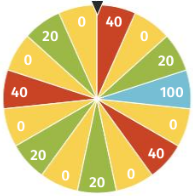
\includegraphics[scale=.7]{roue.png}
    \end{center}
  \end{minipage}
\end{exo}

\begin{exo}
  Un sac contient quatre bougies dont deux sont rouges et deux sont vertes.
  Pierrot sort une à une les quatre bougies. On note $X$ la variable aléatoire
  donnant le rang de la première bougie rouge sortie. Donner la loi de
  probabilité de $X$.
\end{exo}


\begin{exo}
  Une urne contient $20$ billes. Seules deux billes sont gagnantes, les autres
  ne rapportent rien. Pour participer, un joueur doit payer $10$ euros puis
  tirer au hasard deux billes de façon simultanée. Il reçoit alors $30$ euros
  par bille gagnante. On note $G$ la variable aléatoire associant le gain
  algébrique réalisé par un joueur lors d'une partie à ce jeu.
  \begin{enumerate}
    \item Déterminer la loi de probabilité de la variable aléatoire $G$.
    \item Calculer l'espérance de la variable aléatoire $G$ et interpréter le
      résultat obtenu.
  \end{enumerate}
\end{exo}

\begin{exo}
  Après avoir misé une certaine somme d'argent, un joueur lance un dé à six
  faces. Il gagne trois euros s'il obtient un diviseur de six. Quel doit être le
  montant de la mise pour que le jeu soit équitable (c'est-à-dire que
  l'espérance de gain soit nulle) ?
\end{exo}

\begin{exo}~\\
  \begin{minipage}[]{.5\textwidth}
    Pour se rendre au travail, Camille prend le bus. Le trajet comporte quatre
    arrêts. On note $S$ le nombre de fois où le bus s'est effectivement arrêté
    lors du 
  \end{minipage}
  \begin{minipage}[]{.5\textwidth}
\begin{center}
  \renewcommand{\arraystretch}{1.3}
  \begin{tabularx}{1\textwidth}{|c|Y|Y|Y|Y|Y|}
    \hline
    $x_i$ & $0$ & $1$ & $2$ & $3$ & $4$ \\
    \hline
    $P\left( S=x_i \right)$ & $0,05$ & $0,15$ & $0,3$ & $0,35$ & $0,15$ \\
    \hline
  \end{tabularx}
\end{center}
  \end{minipage}
  trajet. Une étude statistique a permis d'établir la loi de probabilité de $S$.
  \begin{enumerate}
    \item Calculer $E(S)$ et interpréter le résultat.
    \item Le trajet direct dure vingt minutes et chaque arrêt rallonge de trois
      minutes la durée du voyage. Soit $T$ la variable aléatoire qui donne la
      durée du trajet.
      \begin{enumerate}
        \item Quelle relation lie $S$ et $T$ ?
        \item En déduire, sur un très grand nombre de jours, le temps de trajet
          moyen mis par Camille pour se rendre au travail.
      \end{enumerate}
  \end{enumerate}
\end{exo}

\begin{exo}~\\%[-5mm]
  \begin{minipage}{.5\textwidth}
    Pour se rendre sur son lieu de travail ($T$) depuis chez lui ($M$), un
    employé a le choix entre plusieurs chemins, tous ayant la même probabilité
    d'être empruntés. Le schéma ci-contre donne les différents itinéraires
    possibles en y indiquant le nombre de feux de circulation sur chaque
    portion. Chaque feu peut être soit vert, soit rouge. On admet que l'employé
    ne passe pas deux fois par le même point lors de
  \end{minipage}
  \begin{minipage}{.5\textwidth}
    \begin{center}
      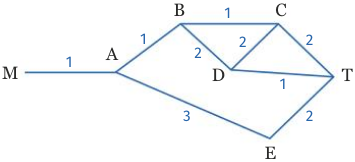
\includegraphics[scale=.7]{chemins.png}
    \end{center}
  \end{minipage}
  son trajet.
  \begin{enumerate}
    \item Donner deux parcours différents permettant d'aller de $M$ à $T$ et
      compter, pour chaque parcours donné, le nombre de feux rencontrés.
  \end{enumerate}
  On note $X$ la variable aléatoire qui donne le nombre de feux de circulation
  rencontrés par cet employé sur les différents parcours.
  \begin{enumerate}
      \setcounter{enumi}{1}
    \item Déterminer la loi de probabilité de $X$.
    \item Calculer $E\left( X \right)$ et interpréter le résultat.
    \item Le trajet sans aucun feu rouge dure $20$ minutes et chaque feu rouge
      rallonge la durée du trajet de trois minutes.
      \begin{enumerate}
        \item Donner le temps de trajet maximal en fonction du nombre de feux
          présents sur le trajet.
        \item L'employé a remarqué que, lors de ses trajets pour se rendre au
          travail, en moyenne un feu sur deux reste vert quand il arrive. Quel
          est le temps de trajet moyen mis par cet employé pour se rendre sur
          son lieu de travail ?
      \end{enumerate}
  \end{enumerate}
\end{exo}

\begin{exo}
  Une usine fabrique des objets destinés à être commercialisés. Sur $100$ objets
  qui sortent de l'usine, en moyenne, quinze ont uniquement le défaut $A$, sept
  ont uniquement le défaut $B$ et trois ont les deux défauts. Le coût de
  production d'un objet est de $150$ euros. Gr\^ace à la garantie, les clients
  peuvent faire réparer leur objet aux frais du fabricant. La réparation du
  défaut $A$ revient à $30$ euros et la réparation du défaut $B$ revient à $40$
  euros. Soit $X$ la variable aléatoire qui associe à un objet choisi au hasard
  dans la production de l'usine, son coût de revient (coût de production $+$
  coût des réparations éventuelles).
  \begin{enumerate}
    \item Déterminer la loi de probabilité de $X$.
    \item Calculer $E(X)$ et interpréter le résultat.
    \item On suppose que tous les objets produits sont vendus.
      \begin{enumerate}
        \item L'usine réalisera-t-elle des bénéfices si elle vend les objets à
          $160$ euros pièce ?
        \item Quel doit être le prix de vente d'un objet pour que l'usine
          réalise un bénéfice moyen de $50$ euros par objet ?
      \end{enumerate}
  \end{enumerate}
\end{exo}

\begin{exo}
  Dans une fête foraine, une machine contient quatre boules noires et deux
  boules blanches. Lorsque l'on introduit un jeton dans la machine, elle tire au
  hasard deux boules successivement et sans remise. Un joueur achète un jeton au
  prix de $5$ euros. Si les deux boules sont blanches, le joueur reçoit $40$
  euros. Si une seule boule est blanche, il reçoit $10$ euros.
  \begin{enumerate}
    \item Traduire la situation par un arbre de probabilité.
    \item Soit $G$ la variable aléatoire donnant le gain algébrique du joueur.
      \begin{enumerate}
        \item Déterminer la loi de probabilité de $G$.
        \item Calculer $E(G)$ et en déduire le gain moyen du forain par partie
          sur un très grand nombre de parties.
      \end{enumerate}
    \item Comme ce jeu n'est pas assez rentable, le forain envisage deux
      solutions : augmenter de $1$ euro le prix du jeton ou bien ajouter
      une boule noire dans la machine. Quelle est la solution la plus
      avantageuse pour le forain ?
  \end{enumerate}
\end{exo}

\end{document}
